% Author: Till Tantau
% Source: The PGF/TikZ manual
\documentclass[a4paper,11pt]{article}
\usepackage[utf8]{inputenc}
\usepackage{listings}
\usepackage{amsmath}    % need for subequations
\usepackage{graphicx}   % need for figures
\usepackage{verbatim}   % useful for program listings
\usepackage{color}      % use if color is used in text
%\usepackage{subfigure}  % use for side-by-side figures
\usepackage{hyperref}   % use for hypertext links, including those to external documents and URLs
\usepackage{url}
\usepackage{float}
\usepackage{todonotes}
\usepackage{tikz}
\usepackage{enumitem}
\usepackage{hyperref}
\usepackage{pdfpages}
\usepackage{caption}
\usepackage{subcaption}
\usepackage{listings}
\usepackage{color}
\usepackage{amsfonts}
\usepackage{latexsym}
\usepackage[T1]{fontenc} % use for allowing < and > in cleartext
\usepackage{fixltx2e}    % use for textsubscript
\usepackage[linesnumbered,boxed,ruled]{algorithm2e}
% \newcommand{\BigO}[1]{\ensuremath{\operatorname{O}\left(#1\right)}}
\newcommand{\BigO}[1]{\ensuremath{\mathop{}\mathopen{}\mathcal{O}\mathopen{}\left(#1\right)}}
\graphicspath{ {./images/} }
\definecolor{mygreen}{rgb}{0,0.6,0}
\definecolor{mygray}{rgb}{0.5,0.5,0.5}
\definecolor{mymauve}{rgb}{0.58,0,0.82}
\lstset{ %
  backgroundcolor=\color{white},   % choose the background color; you must add \usepackage{color} or \usepackage{xcolor}
  basicstyle=\footnotesize,        % the size of the fonts that are used for the code
  breakatwhitespace=false,         % sets if automatic breaks should only happen at whitespace
  breaklines=true,                 % sets automatic line breaking
  captionpos=b,                    % sets the caption-position to bottom
  commentstyle=\color{mygreen},    % comment style
  deletekeywords={...},            % if you want to delete keywords from the given language
  escapeinside={\%*}{*)},          % if you want to add LaTeX within your code
  extendedchars=true,              % lets you use non-ASCII characters; for 8-bits encodings only, does not work with UTF-8
  %frame=single,                    % adds a frame around the code
  keepspaces=true,                 % keeps spaces in text, useful for keeping indentation of code (possibly needs columns=flexible)
  keywordstyle=\color{blue},       % keyword style
  language=Octave,                 % the language of the code
  morekeywords={*,...},            % if you want to add more keywords to the set
  numbers=left,                    % where to put the line-numbers; possible values are (none, left, right)
  numbersep=5pt,                   % how far the line-numbers are from the code
  numberstyle=\tiny\color{mygray}, % the style that is used for the line-numbers
  rulecolor=\color{black},         % if not set, the frame-color may be changed on line-breaks within not-black text (e.g. comments (green here))
  showspaces=false,                % show spaces everywhere adding particular underscores; it overrides 'showstringspaces'
  showstringspaces=false,          % underline spaces within strings only
  showtabs=false,                  % show tabs within strings adding particular underscores
  stepnumber=2,                    % the step between two line-numbers. If it's 1, each line will be numbered
  stringstyle=\color{mymauve},     % string literal style
  tabsize=2,                       % sets default tabsize to 2 spaces
  %title=\lstname                   % show the filename of files included with \lstinputlisting; also try caption instead of title
}

\bibliographystyle{plain}
\begin{document}
\date{TODO DATO}
\title{Eye Tracking\\SIGB Spring 2014}

\author{Marcus Gregersen\\
\texttt{mabg@itu.dk}
\and Martin Faartoft\\
\texttt{mlfa@itu.dk}
\and Mads Westi\\
\texttt{mwek@itu.dk}}
%TODO vejleder og institut
\clearpage\maketitle
\thispagestyle{empty}
\setcounter{page}{1}
\newpage

\section{Introduction}

%billede af øje med navne på de forskellige ting

\section{Pupil Detection}
In this section, we will investigate and compare different techniques for pupil detection.

\subsection{Thresholding}
An obvious first choice of technique, is using a simple threshold to find the pupil, then do connected component (blob) analysis, and finally fit an ellipse on the most promising blobs.

Fig \ref{fig:eye1_threshold_93} shows an example of an image from the 'eye1.avi' sequence and the binary image produced by, using a threshold that blacks out all pixels with intensities above 93. This manages to separate the pupil nicely from the iris.

\begin{figure}[ht]
  \centering
  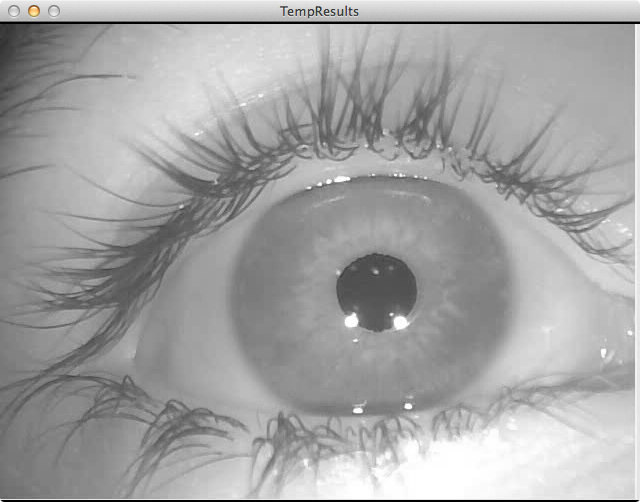
\includegraphics[scale=0.2]{eye1}
  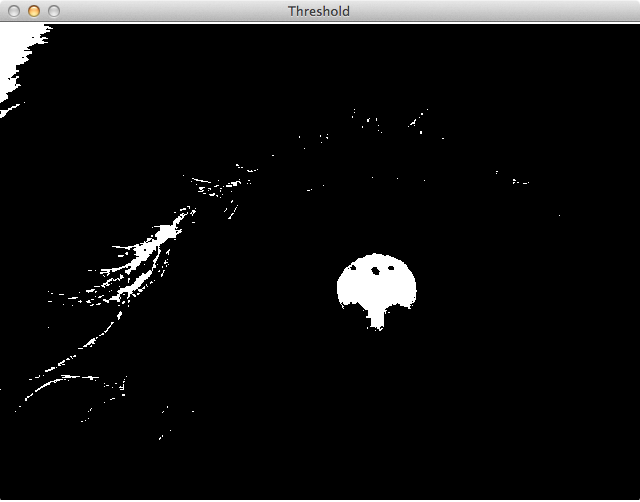
\includegraphics[scale=0.2]{eye1_threshold_93}
  \caption{Thresholding eye1.avi}
  \label{fig:eye1_threshold_93}
\end{figure}

The next step, is to do connected component analysis, and fit an ellipsis through the blobs. As seen in fig \ref{fig:eye1_unfiltered}, this succesfully detects the pupil, but is extremely prone to false positives.

\begin{figure}[ht]
  \centering
  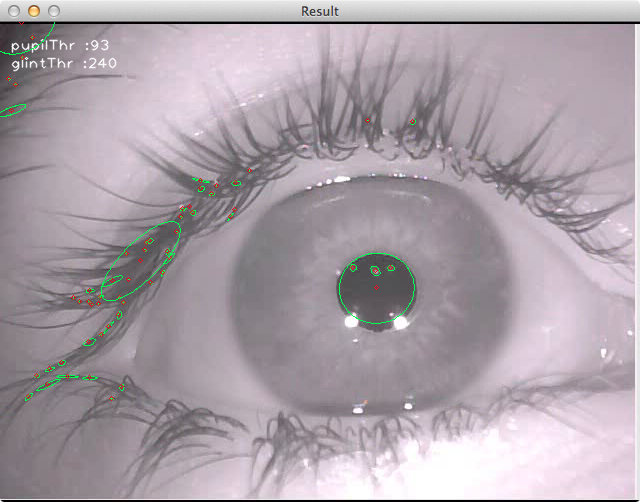
\includegraphics[scale=0.3]{eye1_unfiltered}
  \caption{Fitting ellipses on blobs from eye1.avi (green figures are ellipses fitted through blobs, red dots are the centerpoint of each blob)}
  \label{fig:eye1_unfiltered}
\end{figure}

By experimenting, we find that requiring that the area of the blob lies in the interval $[1000:10000]$, and the extent between $[0.4:1.0]$, we eliminate most false positives on the entire eye1 sequence, while still keeping the true positive.

\paragraph{}
This approach has several problems, however. Note how the true positive on fig \ref{fig:eye1_unfiltered} fails to follow the bottom of pupil correctly. This is due to the glints obscuring part of the boundary between pupil and iris. It also makes some sweeping assumptions:

\paragraph{The pupil has size at least size 1000}
If the person on the sequence leans back slightly, the pupil will shrink and we will fail to detect it.

\paragraph{A threshold of 93 will cleanly separate pupil from iris}
This is true for eye1.avi, but generalizes extremely poorly to the other sequences. If this approach is to be used across multiple sequences recorded in different lighting conditions, the threshold will have to be adjusted by hand for each one.

This problem can be mitigated somewhat with Histogram Equalization. A threshold of 25 on Histogram Equalized images, fares considerably better across several sequences. Note that this will still fail, if parts of the image are significantly darker than the pupil, thereby messing up the equalization.

\begin{figure}[ht]
  \centering
  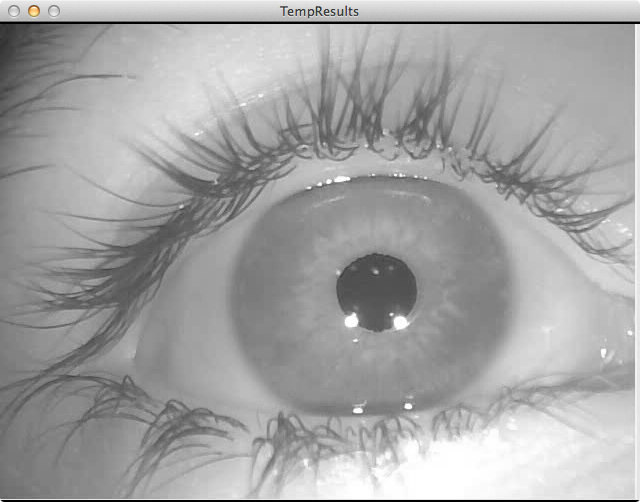
\includegraphics[scale=0.2]{eye1}
  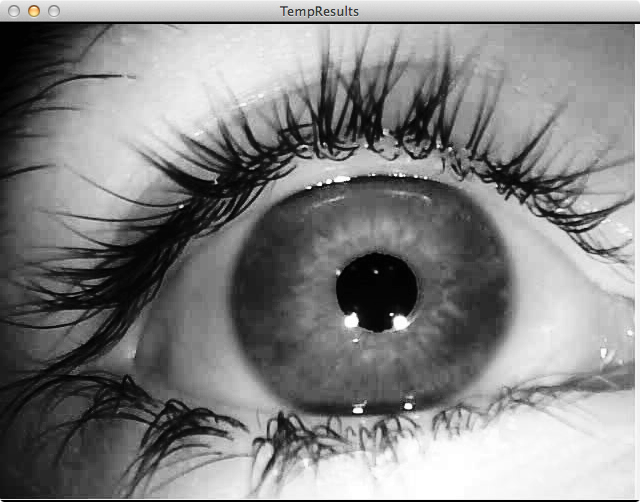
\includegraphics[scale=0.2]{eye1_hist_eq}
  \caption{Eye1 before and after Histogram Equalization}
  \label{fig:eye1_hist_eq}
\end{figure}

\begin{figure}[ht]
  \centering
  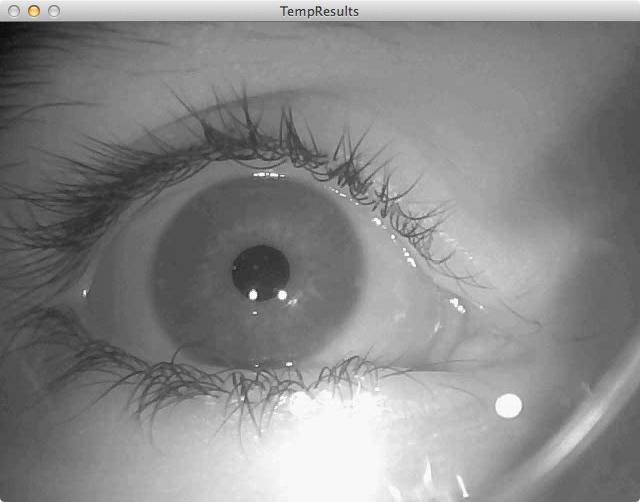
\includegraphics[scale=0.2]{eye3}
  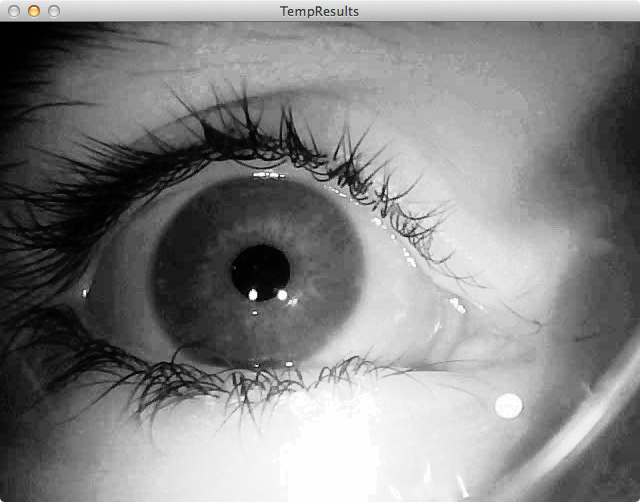
\includegraphics[scale=0.2]{eye3_hist_eq}
  \caption{Eye3 before and after Histogram Equalization}
  \label{fig:eye3_hist_eq}
\end{figure}

\paragraph{Morphology}
Using Morphology, we can improve the detected pupil. The problem with the glints obscuring part of the boundary can be mitigated with the 'closing' operator - used to fill in holes in binary images. Fig \ref{fig:morph} shows binary images before and after applying the closing operator. Notice how the noise inside the pupil is completely removed, and the glints are mostly removed.
A downside to using the closing operation, is that adjacent, sparse structures may merge and resemble circles.

\begin{figure}[ht]
  \centering
  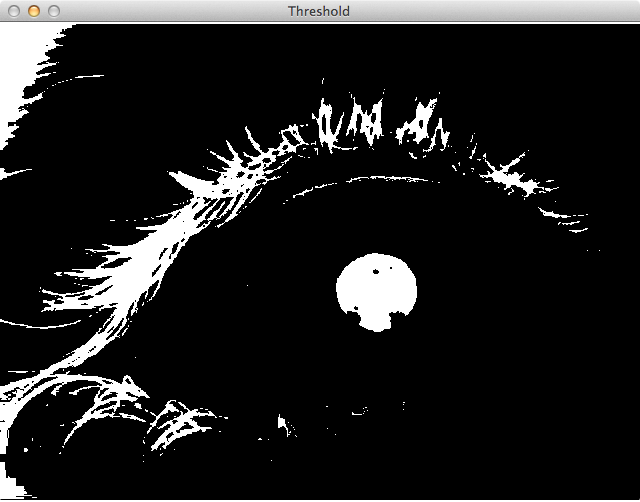
\includegraphics[scale=0.2]{eye1_close_5}
  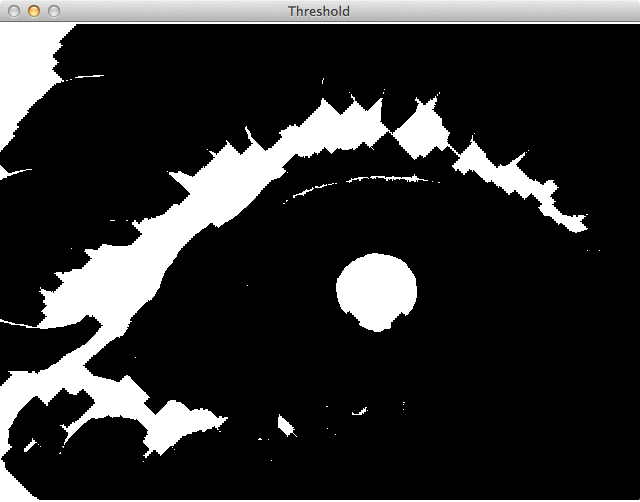
\includegraphics[scale=0.2]{eye1_no_morph}
  \caption{Eye1 before and after Closing (5 iterations, 5x5 CROSS structuring element)}
  \label{fig:morph}
\end{figure}

\paragraph{Tracking} The pupil tracker can be further improved, by using information about the pupil positions from the previous frame. We do it as follows:
\begin{description}
\item[1.]{Search within some threshold distance from each pupil in previous frame}
\item[2.]{One or more pupils were found within the distance, return those}
\item[3.]{No pupils were found within the distance, search the entire image}
\end{description}
Because of the fallback clause in '3', it is very unlikely that the true positive is not detected in each frame. The only case I can think of where this approach fails, is if the pupil is obscured for a frame (subject blinking for example), while a false positive is still detected. In that case, the pupil will improperly detected for as long as the false positive continues to be present.



%current:
%threshold->contour detection->contour filtering->ellipsis detection

%clustering (part 2)

%what assumptions do we make?
%how does it perform, when does it work, what causes it to fail
%test on own sequence

%improvements:
\subsection{Pupil Detection by circular Hough transformation}

In an attempt to make our pupil detection more robust we now investigate the result of applying a
circular hough transformation on the eye images.

The main challenge is finding the correct parameters for the process. We consider the following parameters:

\begin{description}
  \item[Gauss kernel size] The size of the gaussian kernel that is applied to the image before the hough transformation

  \item[$\sigma$ - value] the standard deviation value used to construct the gaussian kernel.

  \item[Accumulator threshold] The minimum cummulative vote thresshold in which some parameters for a circle are considered.

  \item[Minimum and Maxiumum Radius] The minumum and maximum radius of circles to consider.

\end{description}

The next step is to experimentally find the parameters that yields the best result over all sequences.

\begin{figure}[H]
\centering
\begin{subfigure}{.5\textwidth}
  \centering
  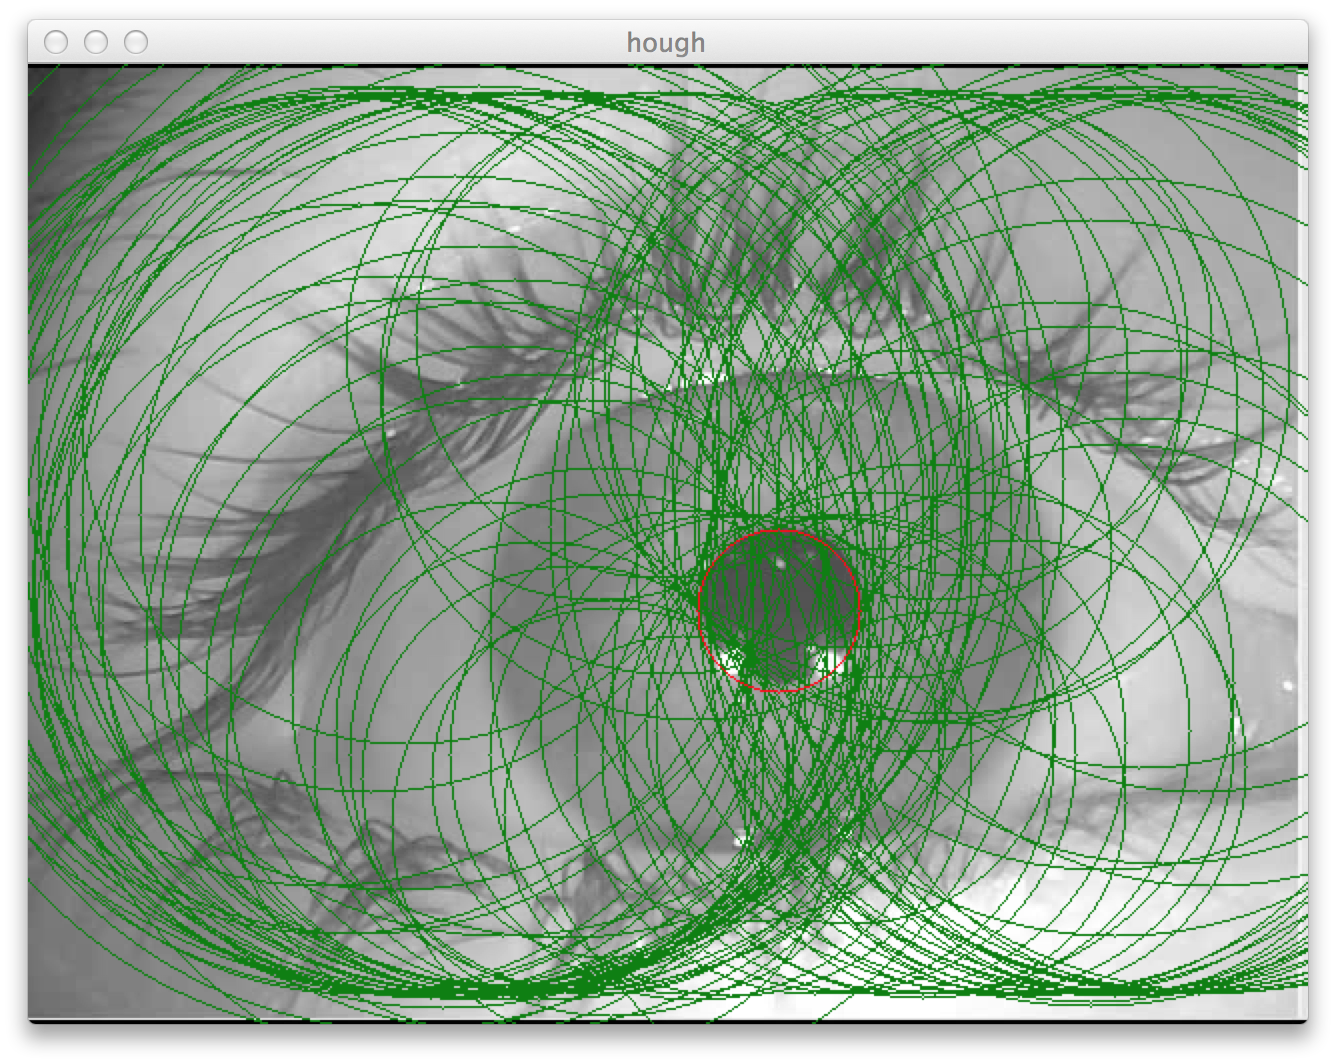
\includegraphics[width=.8\linewidth]{hough100}
  \caption{Accumulator threshold at 100}
  \label{fig:sub1}
\end{subfigure}%
\begin{subfigure}{.5\textwidth}
  \centering
  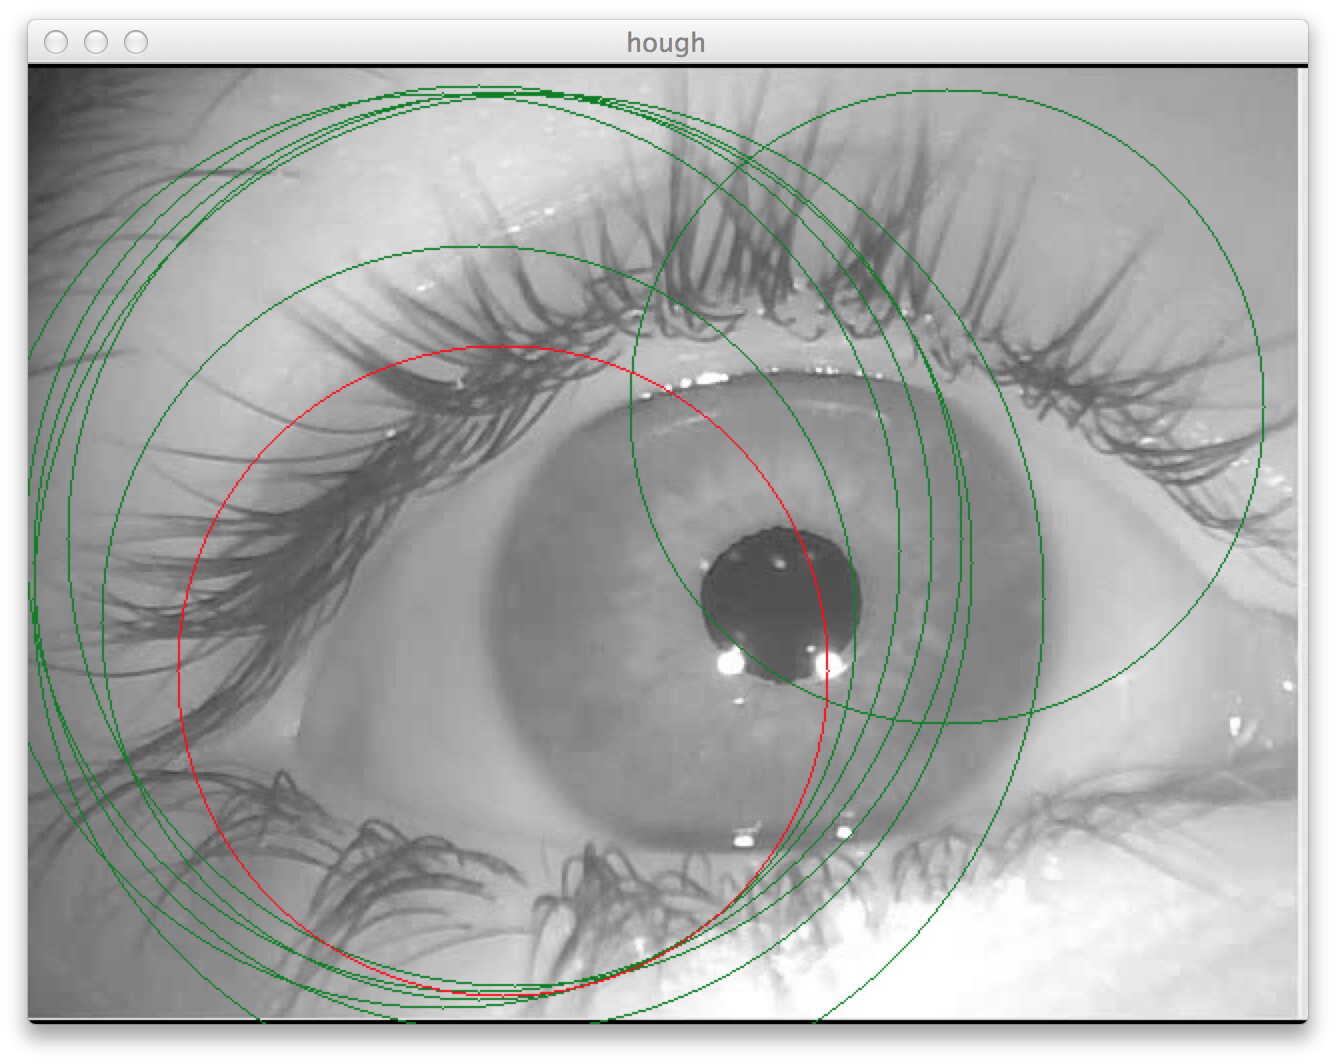
\includegraphics[width=.8\linewidth]{hough150}
  \caption{Accumulator threshold at 150}
  \label{fig:sub2}
\end{subfigure}
\caption{Finding the accumulator threshold values}
\label{fig:test}
\end{figure}

\begin{figure}[H]
\centering
\begin{subfigure}{.5\textwidth}
  \centering
  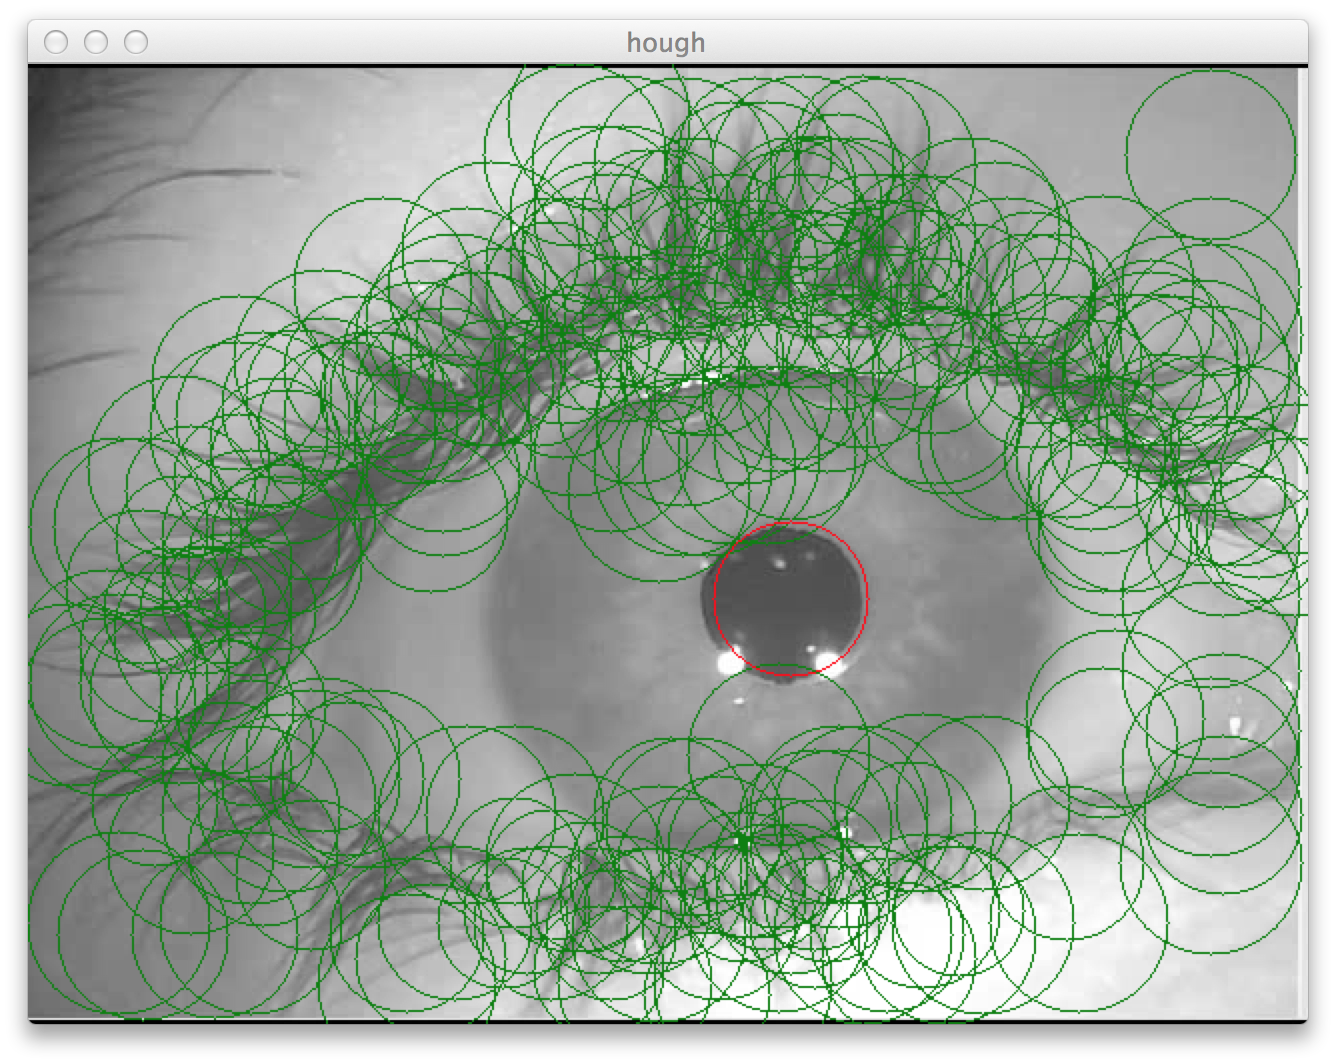
\includegraphics[width=.8\linewidth]{houghk9s9}
  \caption{Size=9, $\sigma$ = 9}
  \label{fig:sub3}
\end{subfigure}%
\begin{subfigure}{.5\textwidth}
  \centering
  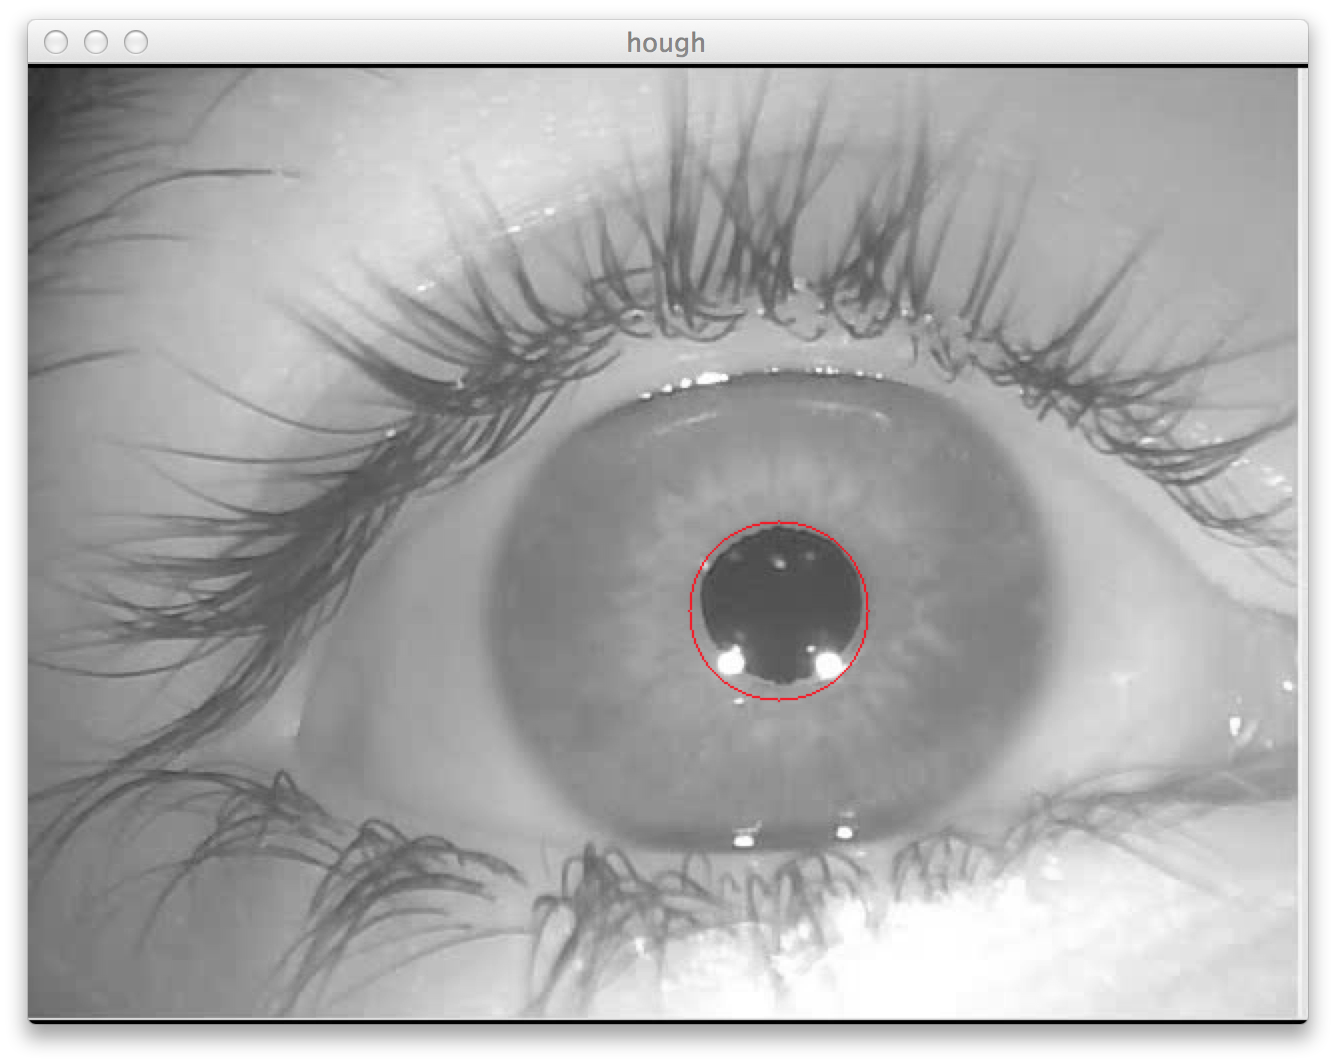
\includegraphics[width=.8\linewidth]{houghk31s9}
  \caption{Size=31, $\sigma$ = 9}
  \label{fig:sub4}
\end{subfigure}
\caption{Preprocessing by smothing with a gaussian kernel}
\label{fig:test2}
\end{figure}

\paragraph{Discussion}
The circular hough transformation yields the most robust pupil detection we have been able to produce so far.

The intuition behind this is that in an ideal setting, where the eye for example is not distorted by perspective, the pupil is going to be near-circular, so the process of hough tranforming and then voting for circles is likely to succeed.

In a non ideal setting, for example in a frame were the eye is seen from the side the pupil is not going to yield the same circular properties, and the process is going to fail.

By preprocessing the image by smooting some of the noise is going to be filtered out. The idea is to choose a kernel that is rougly of the same size as the pupil. In this manner smaller features, such as eye lashes will be smothed away, but still maintaining the pupil feature.

The drawback of setting a constant size for the gaussian kernel is that is is not scale independent. An ideal kernel in some frame may smooth away the pupil in some other frame is the subject moved closer or futher away from the camera.









%Hough-transform for ellipsis fitting/detection
%histogram equalization/normalization for making thresholding more robust across sequences
%experiments with morphology


\section{Glint Detection}
%current:
%threshold->morphology->contour detection->contour filtering->distance from pupil center

%what assumptions do we make?
%how does it perform, when does it work, what causes it to fail
%test on own sequence

%improvements:
%Laplacian?
%hist equal?

\section{Eye Corner Detection}

%what assumptions do we make?
%how does it perform, when does it work, what causes it to fail
%test on own sequence

\section{Iris / Limbus Detection}

%what assumptions do we make?
%how does it perform, when does it work, what causes it to fail
%test on own sequence


\section{Conclusion}

\newpage

\begin{thebibliography}{}

\bibitem{paper:foo}
Foo
      %Sådan her ref'er man en URL
      %\bibitem{lit:json}
      %\url{http://tools.ietf.org/html/rfc4627}
      %Retrieved: 2013-05-02
\end{thebibliography}

%code in appendix
\section*{Appendix}
%\lstinputlisting[language=Python]{../tools/size_estimator.py}


\end{document}
